\documentclass{report}
\usepackage{graphicx} % Required for inserting images
\usepackage{geometry}
\usepackage{amsmath}
\usepackage{mathtools}
\usepackage{amssymb}
\usepackage{kotex}
\usepackage{makecell}
\usepackage{bytefield}
\usepackage{listings}
\usepackage{caption}
\usepackage{subcaption}

\captionsetup{labelformat=empty,labelsep=none,font=small}
\lstset{
    basicstyle=\small\ttfamily,
    commentstyle=\small\ttfamily,
    numbers=left,
    columns=flexible,
    breaklines=true,
    captionpos=b,
    xleftmargin=5.0ex,
    aboveskip=1.0em,
}

\title{CSED551 PA\#1 \\[0.5ex] {\normalsize :Image Filtering}}
\author{\small{20220848 Minsu Sun}}
\date{\small{September 30, 2024}}

\begin{document}

\maketitle

\section*{Problem 1}

\small \textit{(하단의 내용은 \code{gaussianFilter}를 구현하는 내용에 대한 설명을 기술합니다.)}

\subsection*{Algorithm - Primitives}

\begin{lstlisting}[language=Python, caption=Primitive - gaussian1D, firstnumber=75]
def gaussian1D(sigma: float, a: int) -> float:
    """Gaussian distribution function in 1D. This function does not consider constant term of the formula.

    Args:
        sigma (float): standard deviation of gaussian distribution
        a (int): input of gaussian distribution

    Returns:
        float: desired output of 1D gaussian distribution at given `a` without consideration of constant alpha
    """
    # ignored constant term: 1 / sqrt(2\pi\sigma^2)
    # normalizing will make them useless
    return np.exp(-(a**2) / (2 * sigma**2))
\end{lstlisting}

위 코드는 1차원 Gaussian 분포를 계산하는 함수이다.
2차원 Gaussian 분포는 1차원 Gaussian 분포의 곱으로 나타낼 수 있으며, 이는 아래의 과정에 따라 자명한 결과이다.

\begin{flalign*}
    Gaussian_{1D}(x) &= c \cdot e^{\frac{x^2}{2\sigma^2}} &&\\
    Gaussian_{1D}(x) \cdot Gaussian_{1D}(y) &= c \cdot e^{\frac{x^2}{2\sigma^2}} \cdot c \cdot e^{\frac{y^2}{2\sigma^2}} = c^2 \cdot e^{\frac{x^2+y^2}{2\sigma^2}} &&\\
    &= Gaussian_{2D}(x,y) &&\\
    &\,(c = \frac{1}{\sqrt{2\pi\sigma^2}}) &&
\end{flalign*}

이에 따라, 2차원 Gaussian 분포는 1차원 Gaussian 분포의 곱을 이용하여 구할 수 있으므로 2차원 Gaussian 분포를 계산하는 함수는 생략한다.
실제 2차원 Gaussian 분포가 필요한 2차원 Gaussian Filter를 계산하는 함수에서도 1차원 Gaussian Filter를 활용하여 계산하기 때문에 더더욱 2차원 Gaussian 분포를 계산하는 함수의 필요성은 더더욱 낮아진다.
위의 계산식 앞에는 상수항 $c$가 존재하지만, 이후 Gaussian Filter를 생성하면서 정규화할 것이기 때문에 상수항은 무시하여 생성하도록 설계하였다.

\begin{lstlisting}[language=Python, caption=Primitive - build1DGaussianKernel, firstnumber=90]
def build1DGaussianKernel(kernel_size: int, kernel_sigma: float) -> np.ndarray:
    """build 1D gaussian kernel with given kernel size and kernel sigman for gaussian distribution

    Args:
        kernel_size (int): _description_
        kernel_sigma (float): _description_

    Returns:
        np.ndarray: (kernel_size, ) 1D gaussian kernel
    """
    mid = kernel_size // 2
    kernel = np.arange(mid + 1, dtype=np.float32)
    kernel = np.vectorize(lambda x: gaussian1D(sigma=kernel_sigma, a=x))(kernel)
    kernel = np.concatenate((kernel[-1:0:-1], kernel))
    return kernel / np.sum(kernel)
\end{lstlisting}

위에서 기술한 \code{gaussian1D} 함수를 이용하여 1차원 Gaussian Filter를 만들어 반환하는 함수이다.
주어지는 \code{kernel_size}가 홀수이며, 필터는 좌우 대칭을 이루기 때문에, 절반에 대해서만 실제 연산을 진행한 후, 나머지는 이를 복사하여 사용하는 식으로 구현하였다.
Gaussian Filter는 정규화된 상태이므로, Gaussian 분포를 이용해 계산한 이후 전체에 대해 정규화를 진행하여 결과를 반환한다.

\begin{lstlisting}[language=Python, caption=Primitive - build2DGaussianKernel, firstnumber=107]
def build2DGaussianKernel(kernel_size: int, kernel_sigma: float) -> np.ndarray:
    """build 2D gaussian kernel with given kernel size and kernel sigman for gaussian distribution

    Args:
        kernel_size (int): kernel size n of n by n matrix
        kernel_sigma (float): standard deviation of gaussian distribution

    Returns:
        np.ndarray: (kernel_size, kernel_size) 2D gaussian kernel
    """
    # 2D Gaussian kernel is product of 1D Gaussian kernel and its transpose
    g = build1DGaussianKernel(
        kernel_size=kernel_size, kernel_sigma=kernel_sigma
    ).reshape(kernel_size, 1)
    kernel = np.matmul(g, g.T)
    # suppose g is normalized already, result of g * g.T should be normalized, too
    return kernel 
\end{lstlisting}

2차원 Gaussian Filter를 생성하여 반환하는 함수이다.
2차원 Gaussian Filter는 \code{(kernel_size, 1)} 크기의 1차원 Gaussian Filter $f$를 이용해 $f \cdot f^T$의 연산을 통해 얻을 수 있는 점을 생각하여 위에서 구현한 \code{build1DGaussianKernel} 함수를 이용해 구현하였다.
\code{build1DGaussianKernel}과 동일하게 정규화를 진행해야 하지만, 정규화된 행렬의 곱 결과 또한 정규화되므로, 정규화는 생략가능하다.

\subsection*{Algorithm - Main Process}

\begin{lstlisting}[language=Python, caption=filterGaussian, firstnumber=7]
def filterGaussian(
        image: np.ndarray,
        kernel_size: int,
        kernel_sigma: float,
        border_type,
        separable: bool,
    ) -> np.ndarray:
        """**PROBLEM 1: GAUSSIAN FILTERING**
    
        Args:
            image (numpy.ndarray): input RGB image
            kernel_size (int): an odd integer to specify the kernel size.If this is 5, then the actual kernel size is 5x5.
            kernel_sigma (float): a positive real value to control the shape of the filter kernel.
            border_type (_type_): extrapolation method for handling image boundaries. Possible values are: `cv2.BORDER_CONSTANT`, `cv2.BORDER_REPLICATE`, `cv2.BORDER_REFLECT`, `cv2.BORDER_WRAP`, `cv2.BORDER_REFLECT_101`
            separable (bool): Boolean value. If `separable == true`, then the function performs Gaussian filtering using two 1D filters. Otherwise, the function performs Gaussian filtering using a normal 2D convolution operation.
    
        Returns:
            image (np.adarray): The function must return a filtered RGB image.
        """
    
        assert len(image.shape) == 3  # do not accept GrayScale or ARGB image
        assert image.shape[2] == 3  # make sure image has RGB channel
        assert kernel_size % 2 == 1  # kernel size is odd
        assert kernel_sigma > 0  # kernel sigma is positive real number
        assert border_type in [
            cv2.BORDER_CONSTANT,
            cv2.BORDER_REPLICATE,
            cv2.BORDER_REFLECT,
            cv2.BORDER_WRAP,
            cv2.BORDER_REFLECT_101,
        ]
    
        # height, width from original image, not padded image
        height, width, channel = image.shape
        result = np.zeros_like(image)
    
        if kernel_size != 1:
            padding_size = kernel_size // 2
            image = cv2.copyMakeBorder(
                image, padding_size, padding_size, padding_size, padding_size, border_type
            )
    
        if separable:
            kernel = build1DGaussianKernel(kernel_size, kernel_sigma)
            kernel_row = kernel.reshape(1, kernel_size)
            kernel_col = kernel.reshape(kernel_size, 1)
        else:
            kernel = build2DGaussianKernel(kernel_size, kernel_sigma)
    
        for i in range(height):
            for j in range(width):
                for k in range(channel):
                    if separable:
                        # (kernel_size, kernel_size) * (kernel_size, 1) * (1, kernel_size)
                        result[i][j][k] = np.sum(
                            image[i : i + kernel_size, j : j + kernel_size, k]
                            * kernel_col
                            * kernel_row
                        )
                    else:
                        # (kernel_size, kernel_size) * (kernel_size, kernel_size)
                        result[i][j][k] = np.sum(
                            image[i : i + kernel_size, j : j + kernel_size, k] * kernel
                        )
    
        return result
\end{lstlisting}

주어진 \code{image}에 Gaussian Filter를 적용하여 반환하는 함수이다.
과제에서 제시한 조건에 따라 \code{assert}를 이용해 전달받은 매개변수의 조건을 검사한다.

\begin{itemize}
    \item 주어진 이미지는 RGB 이미지이므로, \code{image.shape}는 3개의 원소만을 가져야한다.
    \item 주어진 이미지는 RGB 이미지이므로, \code{image}는 3개의 채널만을 가져야한다. 이외의 경우에는 GrayScale 이미지이거나, ARGB 이미지라고 인식해 오류를 발생한다.
    \item \code{kernel_size}는 홀수로 제한된다.
    \item \code{kernel_sigma}는 양의 실수이다. Python의 타입에 따른 유연성 때문에, 양의 범위에 해당함을 확인한다.
    \item \code{border_type}은 제시된 경우에 대해서만 선택할 수 있으므로, 이를 확인한다.
\end{itemize}

\code{image}로부터 \code{height}, \code{width}, \code{channel}을 따로 저장하고, \code{np.zeros_like}를 이용해 \code{image}의 형태가 같은 변수를 만들어 결과를 담는 변수로 사용한다.
\code{kernel_size}가 \code{1}일 경우, 패딩을 진행할 필요가 없기 때문에, \code{kernel_size}가 \code{1}이 아닌 경우에만 \code{cv2.copyMakeBorder}를 이용해 지정된 \code{border_type}에 따른 패딩을 진행하여 저장한다.
패딩하는 사이즈의 경우, \code{kernel_size=2n+1}에서 모든 방향으로 \code{n}만큼의 패딩이 필요하므로, \code{kernel_size//2}를 사이즈로 사용한다.

이후 filter(이후 kernel이라 칭함)를 준비하는데, 함수의 매개변수 \code{separable}에 따라서 \code{True}일 경우 2차원 Gaussian Kernel, \code{False}일 경우 1차원 Gaussian Kernel을 각 행과 열에 대해 준비한다.
이 때, \code{build1DGaussianKernel}의 반환값은 \code{(kernel_size, )}의 형태이기 때문에, 행과 열 Kernel을 각각 \code{(1, kernel_size)}, \code{(kernel_size, 1)}의 행렬이 되도록 \code{kernel.reshape}을 통해 조정한다.

이 단계까지는 다음과 같은 상태를 만족한다.

\begin{itemize}
    \item \code{image} : \code{(height + 2 * padding_size, width + 2 * padding_size, channel)}의 shape를 가진다.
    \item \code{result} : \code{(height, width, channel)}의 shape를 가진다.
    \item \code{kernel*} : \code{separable} 여부에 따라 \code{kernel_row}와 \code{kernel_col} 혹은 \code{kernel}가 정의된다.
\end{itemize}

준비된 Kernel을 이용하여 이미지와 Convolution 연산을 진행한다.
패딩된 이미지를 각 채널별로 \code{kernel_size}에 맞추어 잘라 이를 \code{numpy}의 broadcasting 연산을 통해서 Convolution을 진행한다.
\code{separable}이 \code{True}일 경우에는 정의된 kernel이 \code{kernel_row}, \code{kernel_col}로 두 가지이므로, 이를 연속해서 연산에 사용한다.

이후 연산이 모두 완료된 이미지를 반환한다.

\subsection*{Input Images}

\begin{figure}[htbp]
    \centering

    \subfloat[color1.jpg]{\includegraphics[width=0.2\linewidth]{../images/input/color1.jpg}}
    \hspace{1pt}
    \subfloat[color2.jpg]{\includegraphics[width=0.2\linewidth]{../images/input/color2.jpg}}
    \hspace{1pt}
    \subfloat[color3.jpg]{\includegraphics[width=0.2\linewidth]{../images/input/color3.jpg}}

    \medskip

    \subfloat[color4.jpg]{\includegraphics[width=0.2\linewidth]{../images/input/color4.jpg}}
    \hspace{1pt}
    \subfloat[color5.jpg]{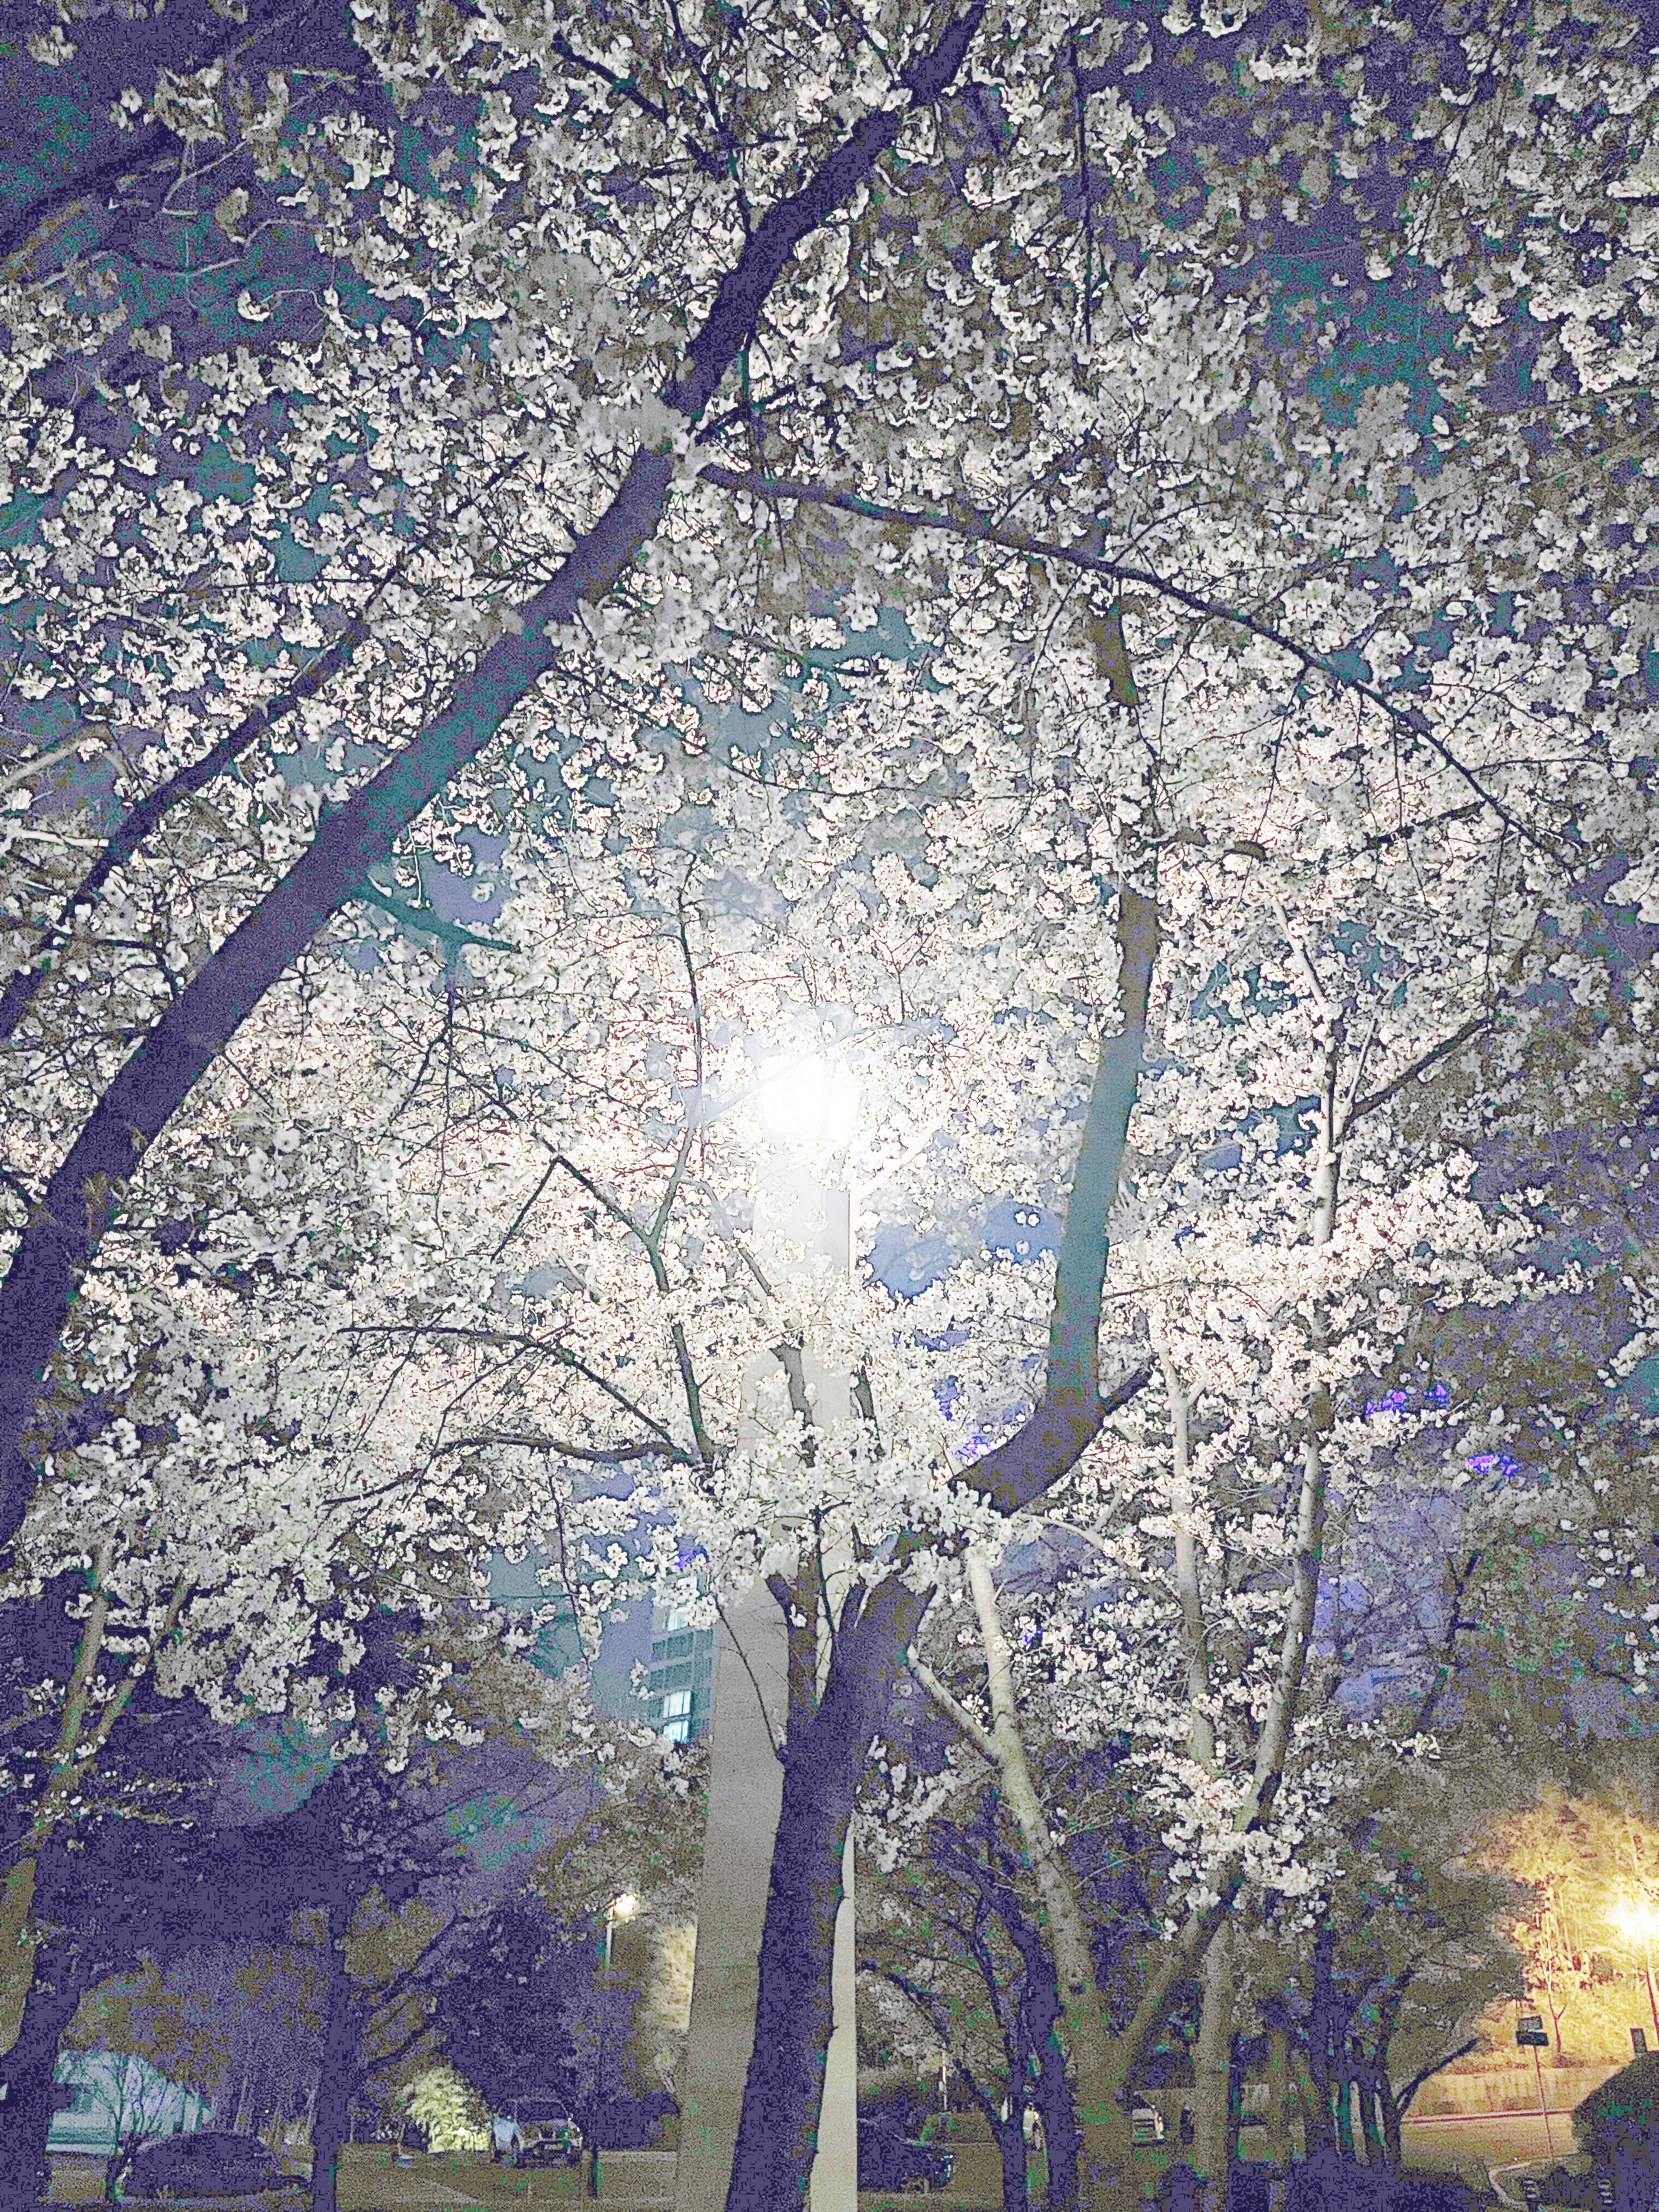
\includegraphics[angle=-90,width=0.2\linewidth]{../images/input/color5.jpg}}
    \hspace{1pt}
    \subfloat[color6.jpg]{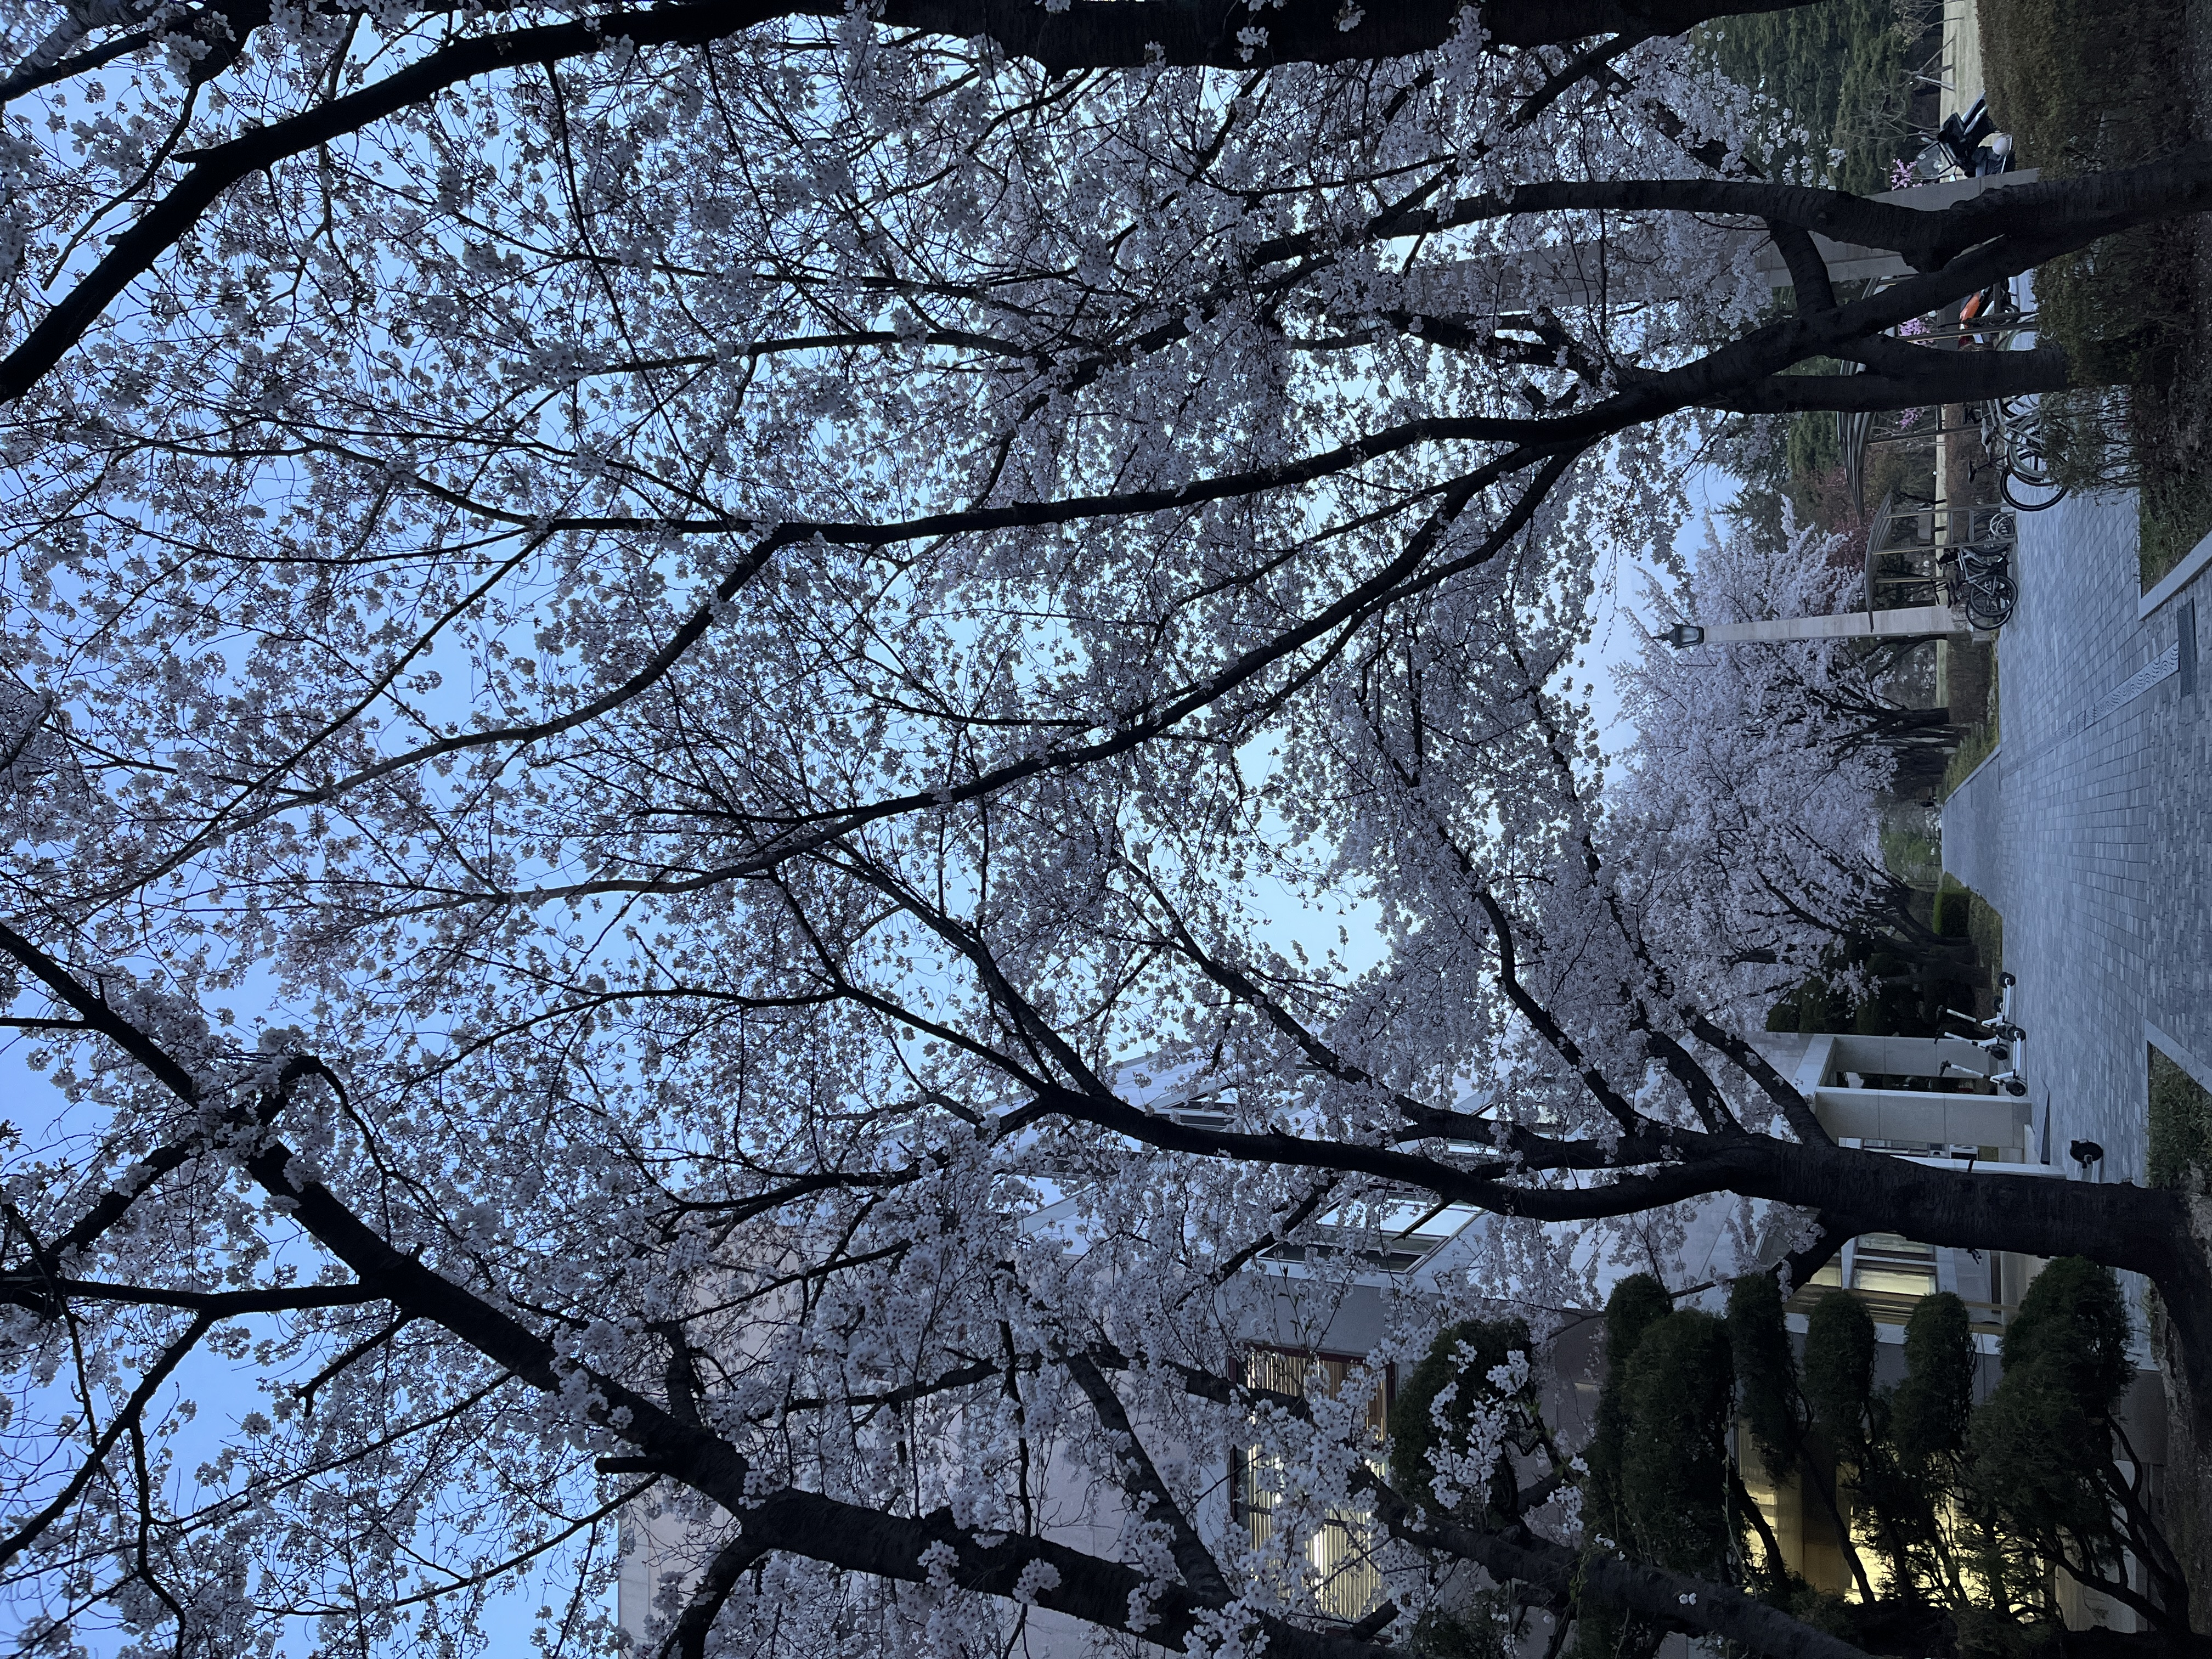
\includegraphics[angle=-90,width=0.2\linewidth]{../images/input/color6.jpg}}

    \caption{Input Images}
\end{figure}

기존 제공된 \code{color1.jpg}, \code{color2.jpg}, \code{color3.jpg} 이외에 \code{color4.jpg}, \code{color5.jpg}, \code{color6.jpg}를 추가하여 사용한다.
추가 이미지는 모두 \code{iPhone 13}에서 촬영된 이미지이다.
이미지의 해상도는 아래와 같다.

\begin{itemize}
    \item \code{color1.jpg} : \code{800px x 450px}
    \item \code{color2.jpg} : \code{800px x 612px}
    \item \code{color3.jpg} : \code{800px x 533px}
    \item \code{color4.jpg} : \code{3024 x 3024px}
    \item \code{color5.jpg} : \code{3024px x 4032px}
    \item \code{color6.jpg} : \code{3024px x 4032px}
\end{itemize}

\subsection*{Input Parameters}

위에서 제시한 이미지를 이용해 \code{fileterGaussian}을 실행할 때, 다음과 같은 파라미터 구성을 이용하여 진행하였다.

\begin{itemize}
    \item \code{border_type} : \code{cv2.BORDER_REPLICATE}, \code{cv2.BORDER_REFLECT}, \code{cv2.BORDER_WRAP}
    \item \code{kernel_size} : \code{1}, \code{25}, \code{45}
    \item \code{kernel_sigma} : \code{0.1}, \code{1}, \code{10}
    \item \code{separable} : \code{True}, \code{False}
\end{itemize}

실행에 실제 사용된 설정은 \code{code/main.py}의 \code{configs['problem1']}에서 확인할 수 있다.

\subsection*{Output Images}

설계된 바에 의하면 결과 이미지의 총 개수는 \code{6 x 3 x 3 x 3 x 2 = 324}로, 현 보고서에 모두 포함하기에는 많아 각 이미지별로 Gaussian Filter 효과가 잘 드러나는 이미지들을 첨부한다.

\noindent \textit{(전체 결과 이미지는 \code{images/output/problem1}에서 확인할 수 있다. 파일 형식은 \code{(input_image)_(kernel_size)_(kernel_sigma)_(border_type)_(separable).jpg}이다.)}

\begin{figure}[htbp]
    \centering

    \subfloat[color1.jpg]{\includegraphics[width=0.2\linewidth]{../images/output/problem1/color1_25_10_replicate_True.jpg}}
    \hspace{1pt}
    \subfloat[color2.jpg]{\includegraphics[width=0.2\linewidth]{../images/output/problem1/color2_25_10_wrap_False.jpg}}
    \hspace{1pt}
    \subfloat[color3.jpg]{\includegraphics[width=0.2\linewidth]{../images/output/problem1/color3_45_10_reflect_True.jpg}}

    \medskip

    \subfloat[color4.jpg]{\includegraphics[width=0.2\linewidth]{../images/output/problem1/color4_45_10_reflect_True.jpg}}
    \hspace{1pt}
    \subfloat[color5.jpg]{\includegraphics[width=0.2\linewidth]{../images/output/problem1/color5_45_10_replicate_True.jpg}}
    \hspace{1pt}
    \subfloat[color6.jpg]{\includegraphics[width=0.2\linewidth]{../images/output/problem1/color6_45_10_wrap_False.jpg}}

    \caption{Output Images}
\end{figure}

각 이미지에서 사용된 파라미터는 다음과 같다. (\code{separable}은 해당 파라미터의 여부에 상관없이 동일한 결과를 내므로 이에 대해서는 기술하지 않는다.)

\begin{itemize}
    \item \code{color1.jpg} : \code{border_type=cv2.BORDER_REPLICATE}, \code{kernel_size=25}, \code{kernel_sigma=10}
    \item \code{color2.jpg} : \code{border_type=cv2.BORDER_WRAP}, \code{kernel_size=25}, \code{kernel_sigma=10}
    \item \code{color3.jpg} : \code{border_type=cv2.BORDER_REFLECT}, \code{kernel_size=45}, \code{kernel_sigma=10}
    \item \code{color4.jpg} : \code{border_type=cv2.BORDER_REFLECT}, \code{kernel_size=45}, \code{kernel_sigma=10}
    \item \code{color5.jpg} : \code{border_type=cv2.BORDER_REPLICATE}, \code{kernel_size=45}, \code{kernel_sigma=10}
    \item \code{color6.jpg} : \code{border_type=cv2.BORDER_WRAP}, \code{kernel_size=45}, \code{kernel_sigma=10}
\end{itemize}

\subsection*{Computation Time}

\noindent {\large\textbf{Kernel Size}}

아래는 Kernel Size에 따른 실행 시간을 표로 나타낸 것이다. 이 때 사용한 파라미터는 \code{cv2.BORDER_REPLICATE}, \code{kernel_sigma=10}, \code{separable=True}이다.

\begin{table*}[h]
    \centering
    \begin{tabular}{@{}cccc@{}}
        \hline
        Input Image & $T_{1}$ & $T_{25}$ & $T_{45}$ \\
        \hline
        color1.jpg & 3.30 & 4.88 & \textbf{6.60} \\
        color2.jpg & 4.28 & 6.29 & \textbf{9.05} \\
        color3.jpg & 3.71 & 5.50 & \textbf{7.82} \\
        color4.jpg & 81.64 & 125.04 & \textbf{173.23} \\
        color5.jpg & 106.95 & 159.21 & \textbf{247.01} \\
        color6.jpg & 106.73 & 158.94 & \textbf{226.98} \\
      \hline
    \end{tabular}
    \caption{Computational Time Depending on Kernel Size}
\end{table*}

Kernel Size가 커짐에 따라서 실행 시간이 늘어나는 것을 확인할 수 있으며, 입력 이미지의 해상도에 따라서도 실행 시간이 달라지는 것을 확인할 수 있었다.

\noindent {\large\textbf{Separable}}

아래는 Separable 여부에 따른 실행 시간을 표로 나타낸 것이다. 이 때 사용한 파라미터는 \code{cv2.BORDER_REPLICATE}, \code{kernel_size=45}, \code{kernel_sigma=10}이다.

\begin{table*}[h]
    \centering
    \begin{tabular}{@{}ccc@{}}
        \hline
        Input Image & $T_{True}$ & $T_{False}$ \\
        \hline
        color1.jpg & 6.60 & \textbf{4.54} \\
        color2.jpg & 9.05 & \textbf{6.17} \\
        color3.jpg & 7.82 & \textbf{5.73} \\
        color4.jpg & 173.23 & \textbf{121.22} \\
        color5.jpg & 247.01 & \textbf{166.04} \\
        color6.jpg & 226.98 & \textbf{156.56} \\
        \hline
    \end{tabular}
    \caption{Computational Time Depending on Separable}
\end{table*}

Separable이 \code{False}인 경우에 실행 시간이 감소하는 것을 확인할 수 있었으며, 이를 통해 1차원 Gaussian Filter를 적용하는 것보다 2차원 Gaussian Filter를 적용하는 것이 훨씬 Computational Cost를 줄인다는 것을 확인할 수 있다.

\noindent {\large\textbf{Discussion - Parameters \& Computation Time}}

앞선 Computation Time 결과를 통해, Kernel Size에 따라 실행 시간이 오래 걸리는 것을 확인할 수 있었다.
Kernel Sigma나 Border Type에 따라서는 실제 연산 횟수가 변화하지 않기 때문에 실행 시간이 달라지지 않는다.
Separable의 경우를 통해, 2D Gaussian Filter를 적용하는 것이 1D Gaussian Filter를 적용하는 것보다 더 적은 연산 횟수를 통해 빠른 실행이 가능하다는 것을 확인할 수 있었다.
파라미터 이외에도 입력 이미지의 해상도에 따라서 실행 시간이 오래 걸리는 것 또한 확인할 수 있었다.

결과를 통해 다음과 같이 연산 시간에 미치는 요소들을 정리할 수 있다.

\begin{itemize}
    \item Kernel Size: \textbf{Kernel Size가 큰 Filter를 사용할수록 연산 시간이 늘어난다}.
    \item Separable: \textbf{2D Gaussian Filter를 적용하는 것이 1D Gaussian Filter를 2번 적용하는 것보다 더 빠른 실행을 보인다}.
    \item Image Size: 큰 이미지일수록 연산이 더 오래걸린다.
\end{itemize}

\subsection*{Filter Visualization}

\noindent {\large\textbf{Visualization}}

실행에서 사용된 파라미터 조합에 따른 Filter를 시각화한 결과는 아래와 같다. (시각화에 대한 상세 코드는 \code{code/main.py}의 \code{problem1_supplementary} 함수에서 확인할 수 있다.)

\begin{figure}[htbp]
    \centering

    \subfloat{\includegraphics[width=0.2\linewidth]{../images/output/problem1/supplementary/1_0.1.png}}
    \subfloat{\includegraphics[width=0.2\linewidth]{../images/output/problem1/supplementary/1_1.png}}
    \subfloat{\includegraphics[width=0.2\linewidth]{../images/output/problem1/supplementary/1_10.png}}

    \medskip

    \subfloat{\includegraphics[width=0.2\linewidth]{../images/output/problem1/supplementary/25_0.1.png}}
    \subfloat{\includegraphics[width=0.2\linewidth]{../images/output/problem1/supplementary/25_1.png}}
    \subfloat{\includegraphics[width=0.2\linewidth]{../images/output/problem1/supplementary/25_10.png}}

    \medskip

    \subfloat{\includegraphics[width=0.2\linewidth]{../images/output/problem1/supplementary/45_0.1.png}}
    \subfloat{\includegraphics[width=0.2\linewidth]{../images/output/problem1/supplementary/45_1.png}}
    \subfloat{\includegraphics[width=0.2\linewidth]{../images/output/problem1/supplementary/45_10.png}}

    \caption{Filter Visualization}
\end{figure}

\noindent {\large\textbf{Discussion - Kernel Size \& $\sigma$}}

같은 \code{kernel_sigma}에서 \code{kernel_size}에 따른 필터를 확인하였을 때, 필터별로 영향을 받는 부분(값이 높은, 시각화 결과에서 하얀색이 많이 보이는)의 분포가 달라지는 것을 확인할 수 있다.
\code{kernel_sigma=10}인 경우 \code{kernel_size=45}에서는 골고루 필터의 전체 범위에 영향을 주는 모습을 볼 수 있지만, \code{kernel_size=25}에서는 다소 너무 많은 부분에서 영향을 주는 것을 확인할 수 있다.

\textbf{
    이에 따라서, 주어진 \code{kernel_size} 혹은 \code{kernel_sigma}에 따라서 올바른 파라미터를 결정하여 필터의 전체 영역에 골고루 영향을 미칠 수 있도록 선택하는 것이 좋아보인다.
    다만, \code{kernel_size}가 큼에도 Gaussian Filter 효과가 두드러지지 않는 케이스가 존재하는데(\code{color4.jpg}, \code{color5.jpg}, \code{color6.jpg}), 이는 이미지의 해상도에 따른 차이이다.
    따라서, \code{kernel_size}는 입력 이미지의 크기에 맞추어 적당한 값을 선택하고, 이를 토대로 필터의 전반적인 부분에 영향을 미칠 수 있는 적당한 \code{kernel_sigma}를 찾는 것이 최적의 방법으로 생각된다.
}

위에서 제시한 시각화 결과 중에서는 \code{kernel_size=45} \code{kernel_sigma=10}인 경우의 필터가 이를 잘 나타내고 있다고 생각되며, \code{kernel_size=25}인 경우에는 \code{kernel_sigma=7} 부근에서 적절한 결과를 보일 것으로 생각된다.

\subsection*{Border Types}

\noindent {\large\textbf{Result}}

아래는 \code{border_type}에 따른 결과 비교이다. 다른 파라미터의 경우, \code{kernel_size=45}, \code{kernel_sigma=10}를 사용하였다.

\begin{figure}[htbp]
    \centering

    \subfloat[color1 - Reflect]{\includegraphics[width=0.2\linewidth]{../images/output/problem1/color1_45_10_reflect_True.jpg}}
    \hspace{1pt}
    \subfloat[color1 - Replicate]{\includegraphics[width=0.2\linewidth]{../images/output/problem1/color1_45_10_replicate_True.jpg}}
    \hspace{1pt}
    \subfloat[color1 - Wrap]{\includegraphics[width=0.2\linewidth]{../images/output/problem1/color1_45_10_wrap_True.jpg}}

    \medskip

    \subfloat[color2 - Reflect]{\includegraphics[width=0.2\linewidth]{../images/output/problem1/color2_45_10_reflect_True.jpg}}
    \hspace{1pt}
    \subfloat[color2 - Replicate]{\includegraphics[width=0.2\linewidth]{../images/output/problem1/color2_45_10_replicate_True.jpg}}
    \hspace{1pt}
    \subfloat[color2 - Wrap]{\includegraphics[width=0.2\linewidth]{../images/output/problem1/color2_45_10_wrap_True.jpg}}

    \medskip

    \subfloat[color3 - Reflect]{\includegraphics[width=0.2\linewidth]{../images/output/problem1/color3_45_10_reflect_True.jpg}}
    \hspace{1pt}
    \subfloat[color3 - Replicate]{\includegraphics[width=0.2\linewidth]{../images/output/problem1/color3_45_10_replicate_True.jpg}}
    \hspace{1pt}
    \subfloat[color3 - Wrap]{\includegraphics[width=0.2\linewidth]{../images/output/problem1/color3_45_10_wrap_True.jpg}}

    \caption{Result of Different Border Types}
\end{figure}

(추가로 사용한 \code{color4.jpg}, \code{color5.jpg}, \code{color6.jpg}의 결과는 위의 3가지 이미지에 비해 차이가 뚜렷하지 않아 생략한다. 이는 입력 이미지의 크기가 나머지에 비해 너무 큰 것으로 판단된다.)

\noindent {\large\textbf{Discussion - Best \& Worst Border Type}}

우선 각 Border Type에 따른 패딩 내용은 다음과 같다.

\begin{itemize}
    \item \code{Reflect} : 가장자리의 이미지를 좌우반전 혹은 상하반전을 통하여 패딩한다.
    \item \code{Replicate} : 가장자리의 픽셀들을 복제하여 패딩한다.
    \item \code{Wrap} : 가장자리의 정반대편에 위치하는 이미지를 이용하여 패딩한다.
\end{itemize}

각 Border Type별 패딩 결과 예시는 아래와 같다.

\begin{figure}[h]
    \centering
    \includegraphics[width=0.6\linewidth]{../images/ref/image1.png}
    \caption{Example of Padding on Various Border Type}
\end{figure}

위의 Border Type에 따른 Gaussian Filtering 결과를 보면, Wrap을 이용한 Border Type의 경우 이미지에 따라서 결과 이미지의 테두리에 검은 음영이 지는 것을 확인할 수 있으며 이는 특히 \code{color1 - Wrap}에서 잘 드러난다(이미지 상단 모서리).
이는 반대편 테두리에 상대적으로 어두운 색이 존재할 경우 어두운 색이 이미지를 패딩하는 과정에 포함되기 때문에, 결과적으로 Gaussian Filtering을 진행할 때도 해당 색이 반영되어 나타나는 결과이다.
반대로 반대편에 상대적으로 밝은 색이 존재할 경우에는 하얀 음영이 생기며, 이 또한 \code{color1 - Wrap}에서 확인할 수 있다(이미지 하단 모서리).

이와 같은 생각을 바탕으로 아래와 같이 Best와 Worst를 선정하였다.

\begin{itemize}
    \item \textbf{Best}: \code{Replicate} - 다른 \code{Wrap}이나 \code{Reflect}에 비해, 가장자리의 색깔을 가장 잘 패딩할 수 있기 때문에, 의도하지 않은 영향을 최소화 할 수 있어 이를 Best로 선정한다.
    \item \textbf{Worst}: \code{Wrap} - 위에서 언급한 대로, 반대편의 상대적으로 다른 색깔이 존재할 경우 의도치 않게 영향을 받게 되기 때문에, Wrap을 Worst로 선정한다.
\end{itemize}

Reflect의 경우, 가장자리는 아니더라도, 가장자리에 상대적으로는 근접한 픽셀이 결국 큰 사이즈의 패딩을 진행할 때 영향을 주게 되어, Wrap의 부작용과 같은 결과를 낼 수 있어 Best로 선정하지 않았다.
이에 따라, 가장자리 근처에서 급격한 색의 변화가 존재할 경우 부작용이 발생할 것으로 생각된다.

\newpage

\section*{Problem 2}

\subsection*{Algorithm - Primitives}

\begin{lstlisting}[language=Python, caption=Primitive - histogramEqulizationSingleChannel, firstnumber=150]
def histogramEqulizationSingleChannel(image: np.ndarray) -> np.ndarray:
    """histogram equalization on single channel

    Args:
        image (np.ndarray): input image of (height, width), this should be single channel image

    Returns:
        np.ndarray: histogram equalized image, same size as input image
    """
    assert len(image.shape) == 2

    hist, _ = np.histogram(image.flatten(), 256, [0, 256])
    chf = hist.cumsum()  # cumulative histogram function
    coef = 255 / chf[-1]  # transformation coefficient
    return np.vectorize(lambda p: int(coef * chf[p]))(image)
\end{lstlisting}

1개의 채널에 대하여 Histogram Equalization을 진행한다.
\code{assert}를 이용하여 주어진 \code{image}의 형태가 1개 채널의 이미지인지 검사한다.
이후, \code{numpy.histogram}을 이용하여 이미지의 히스토그램을 계산하여 저장한다.
각 픽셀의 최대값은 256이므로 히스토그램의 구간 또한 \code{[0,256]}으로 설정하여 계산한다.
구한 히스토그램을 기반으로 Cumulative Sum을 계산하여, Cumulative Histogram Function을 구한다.
이때, Cumulative Histogram Function의 마지막 값은 전체 픽셀의 개수이므로, 이는 \code{width x height} 결과와 같다.
이미 Cumulative Function을 통해 구하였으므로, 이를 이용하여 Equlization 계수로 사용한다.
주어진 image에 위에서 구한 Equlization 계수를 이용하여 Transform 함수를 \code{numpy.vectorize}로 적용시켜 결과를 반환한다.

\subsection*{Algorithm - Main Process}

\begin{lstlisting}[language=Python, caption=Primitive - histogramEqualization, firstnumber=129]
def histogramEqualization(image: np.ndarray) -> np.ndarray:
    """**PROBLEM 2: HISTOGRAM EQUALIZATION**

    Args:
        image (np.ndarray): input image, it should be grayscale or (a)rgb image

    Returns:
        np.ndarray: histogram equalized image, same size as input image
    """
    assert (
        len(image.shape) == 3 or len(image.shape) == 2
    )  # image should be (A)RGB or GRAYSCALE

    if len(image.shape) == 2:  # GRAYSCALE
        return histogramEqulizationSingleChannel(image)

    for c in range(image.shape[2]):
        image[:, :, c] = histogramEqulizationSingleChannel(image[:, :, c])
    return image
\end{lstlisting}

주어진 image의 \code{shape}를 통해 채널이 존재하는 이미지이거나 채널이 존재하지 않는 흑백 이미지일 수 있도록 \code{assert}로 검사한다.
\code{shape}이 \code{(height, width)}인 흑백 이미지의 경우, 단일 채널이며, 이에 대한 Histogram Equlization은 위의 \code{histogramEqulizationSingleChannel}을 이용하여 계산 후 반환한다.
이외에는 채널이 1개 이상 존재하는 이미지이므로, 각 채널에 대한 이미지를 추출하여 각각에 대해 Histogram Equlization을 진행한 후, 이를 각 채널에 다시 저장한다.
이후 계산된 결과를 반환하여 마무리한다.

\subsection*{Input Images}

\begin{figure}[htbp]
    \centering

    \subfloat[gray1.jpg]{\includegraphics[width=0.2\linewidth]{../images/input/gray1.jpg}}
    \hspace{1pt}
    \subfloat[gray2.jpg]{\includegraphics[width=0.2\linewidth]{../images/input/gray2.jpg}}
    \hspace{1pt}
    \subfloat[gray3.jpg]{\includegraphics[width=0.2\linewidth]{../images/input/gray3.jpg}}

    \medskip

    \subfloat[gray4.jpg]{\includegraphics[width=0.2\linewidth]{../images/input/gray4.jpg}}
    \hspace{1pt}
    \subfloat[gray5.jpg]{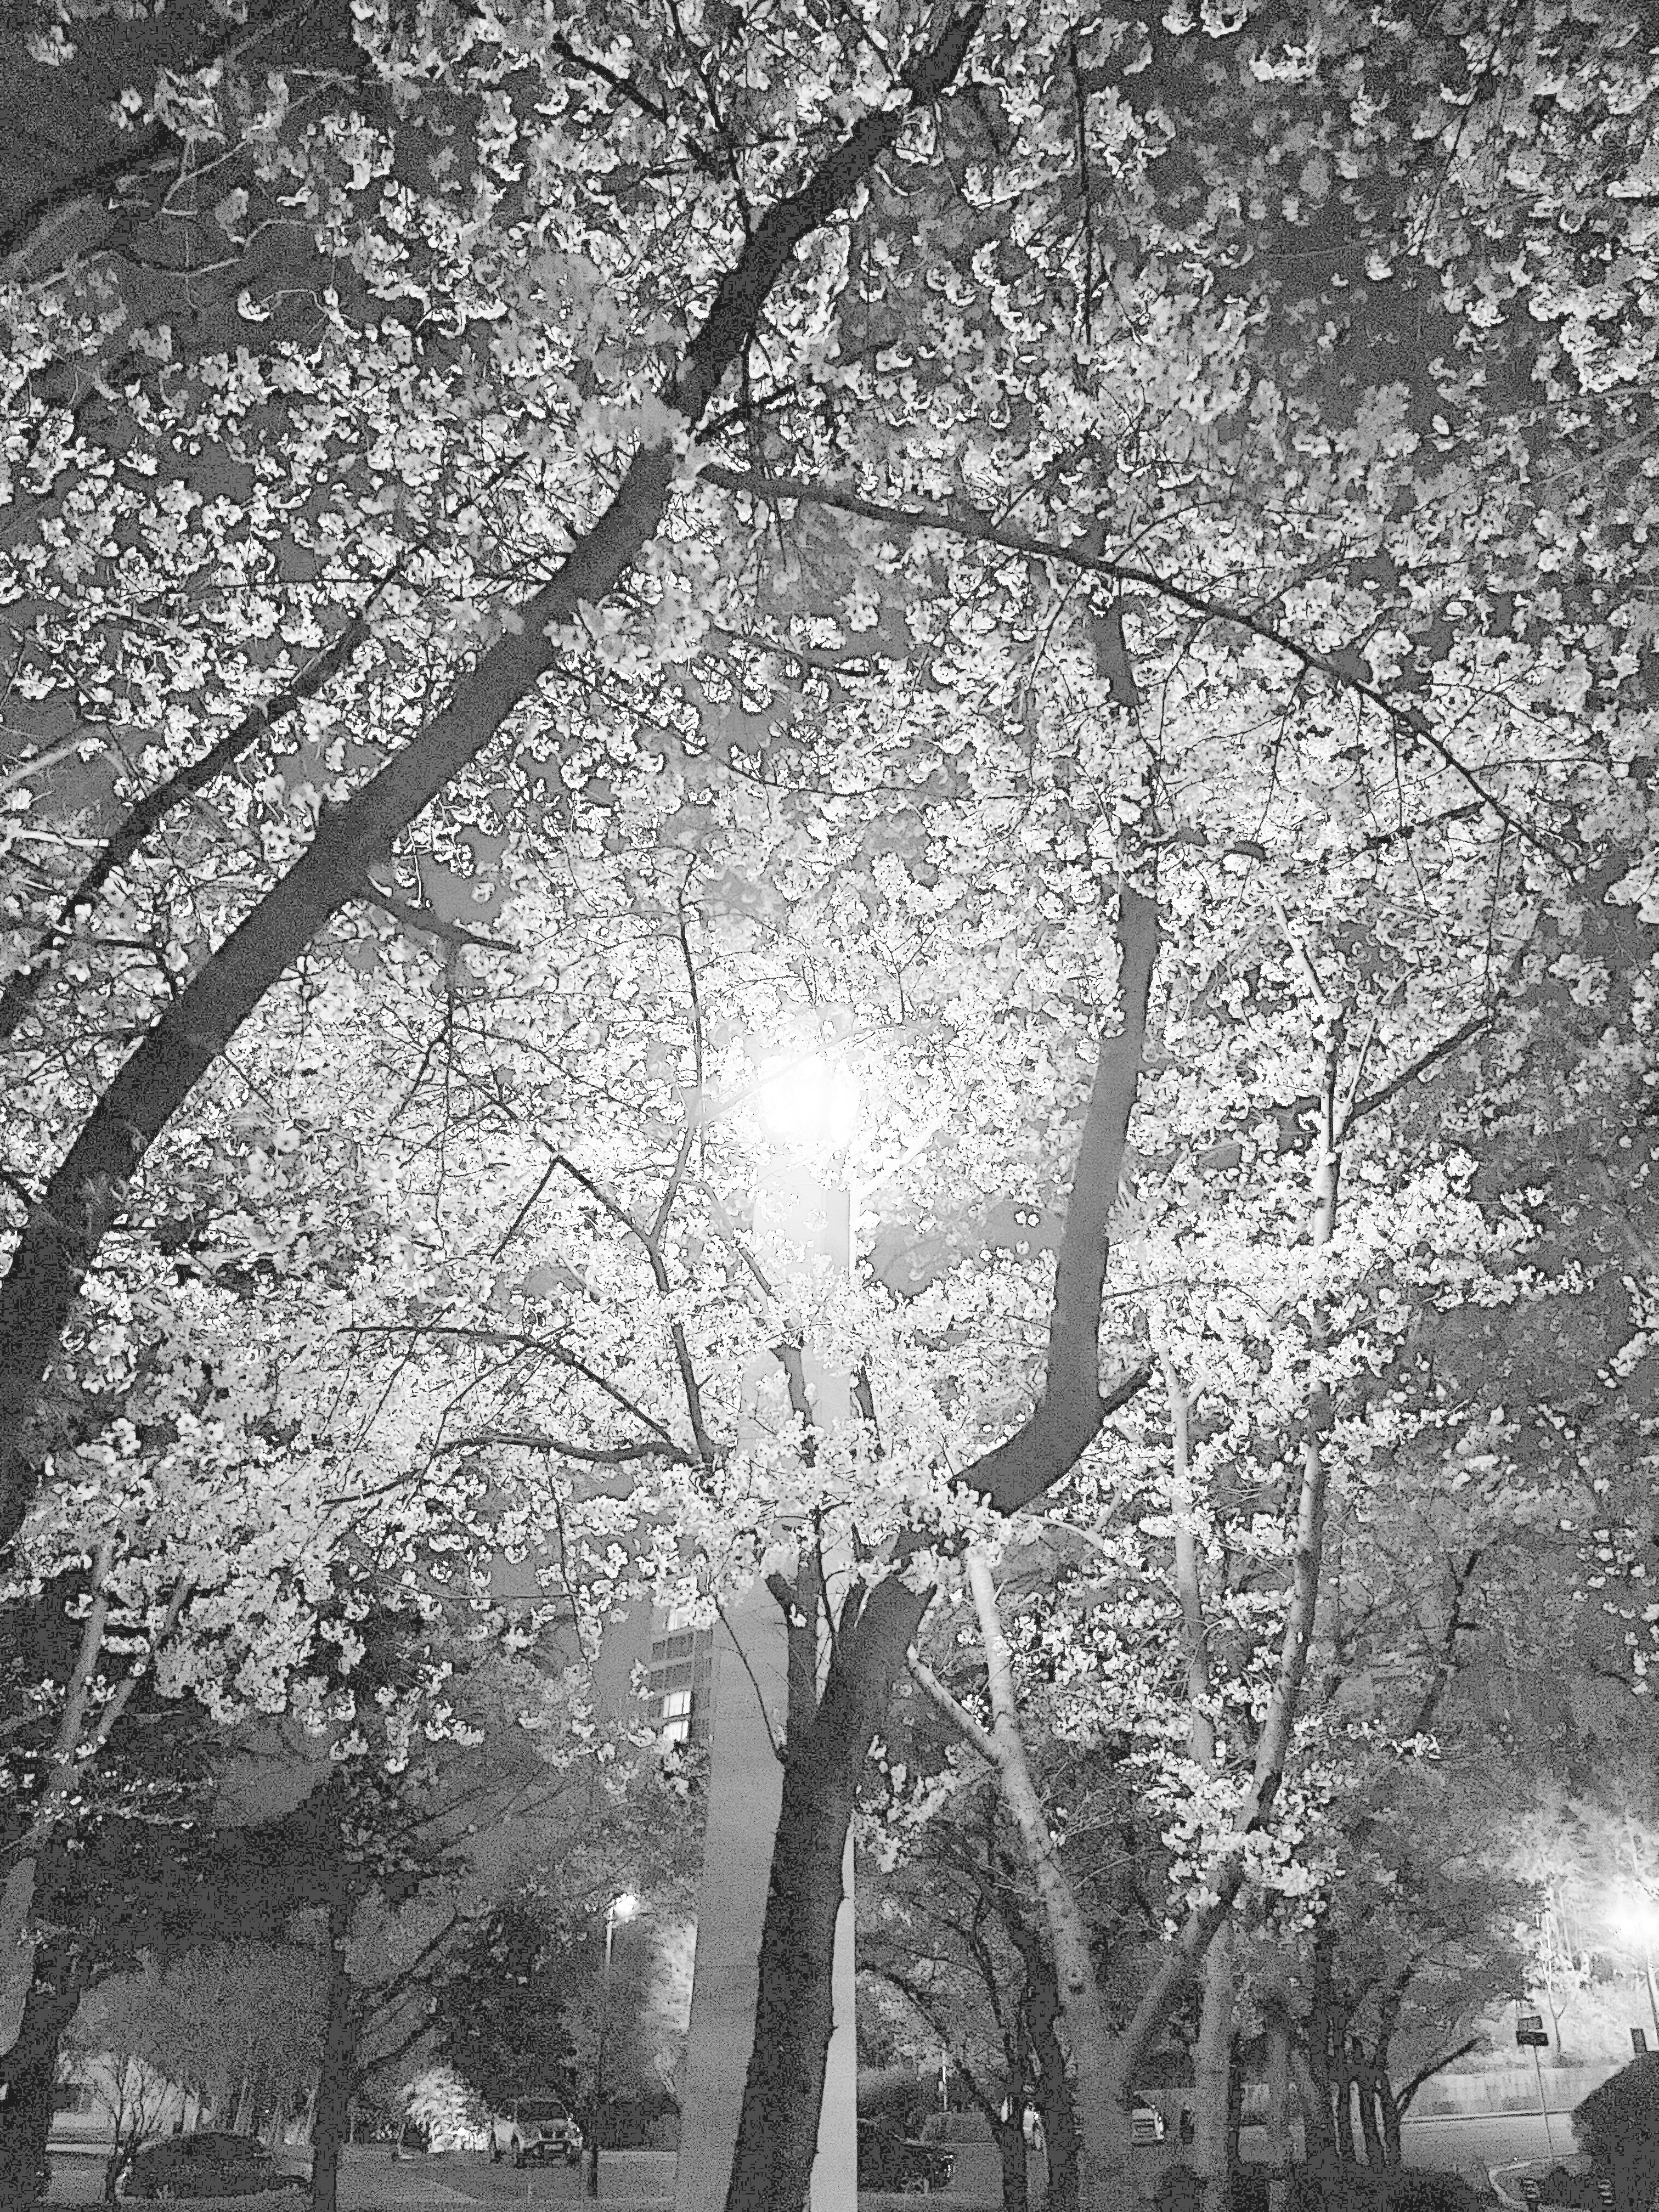
\includegraphics[width=0.2\linewidth]{../images/input/gray5.jpg}}
    \hspace{1pt}
    \subfloat[gray6.jpg]{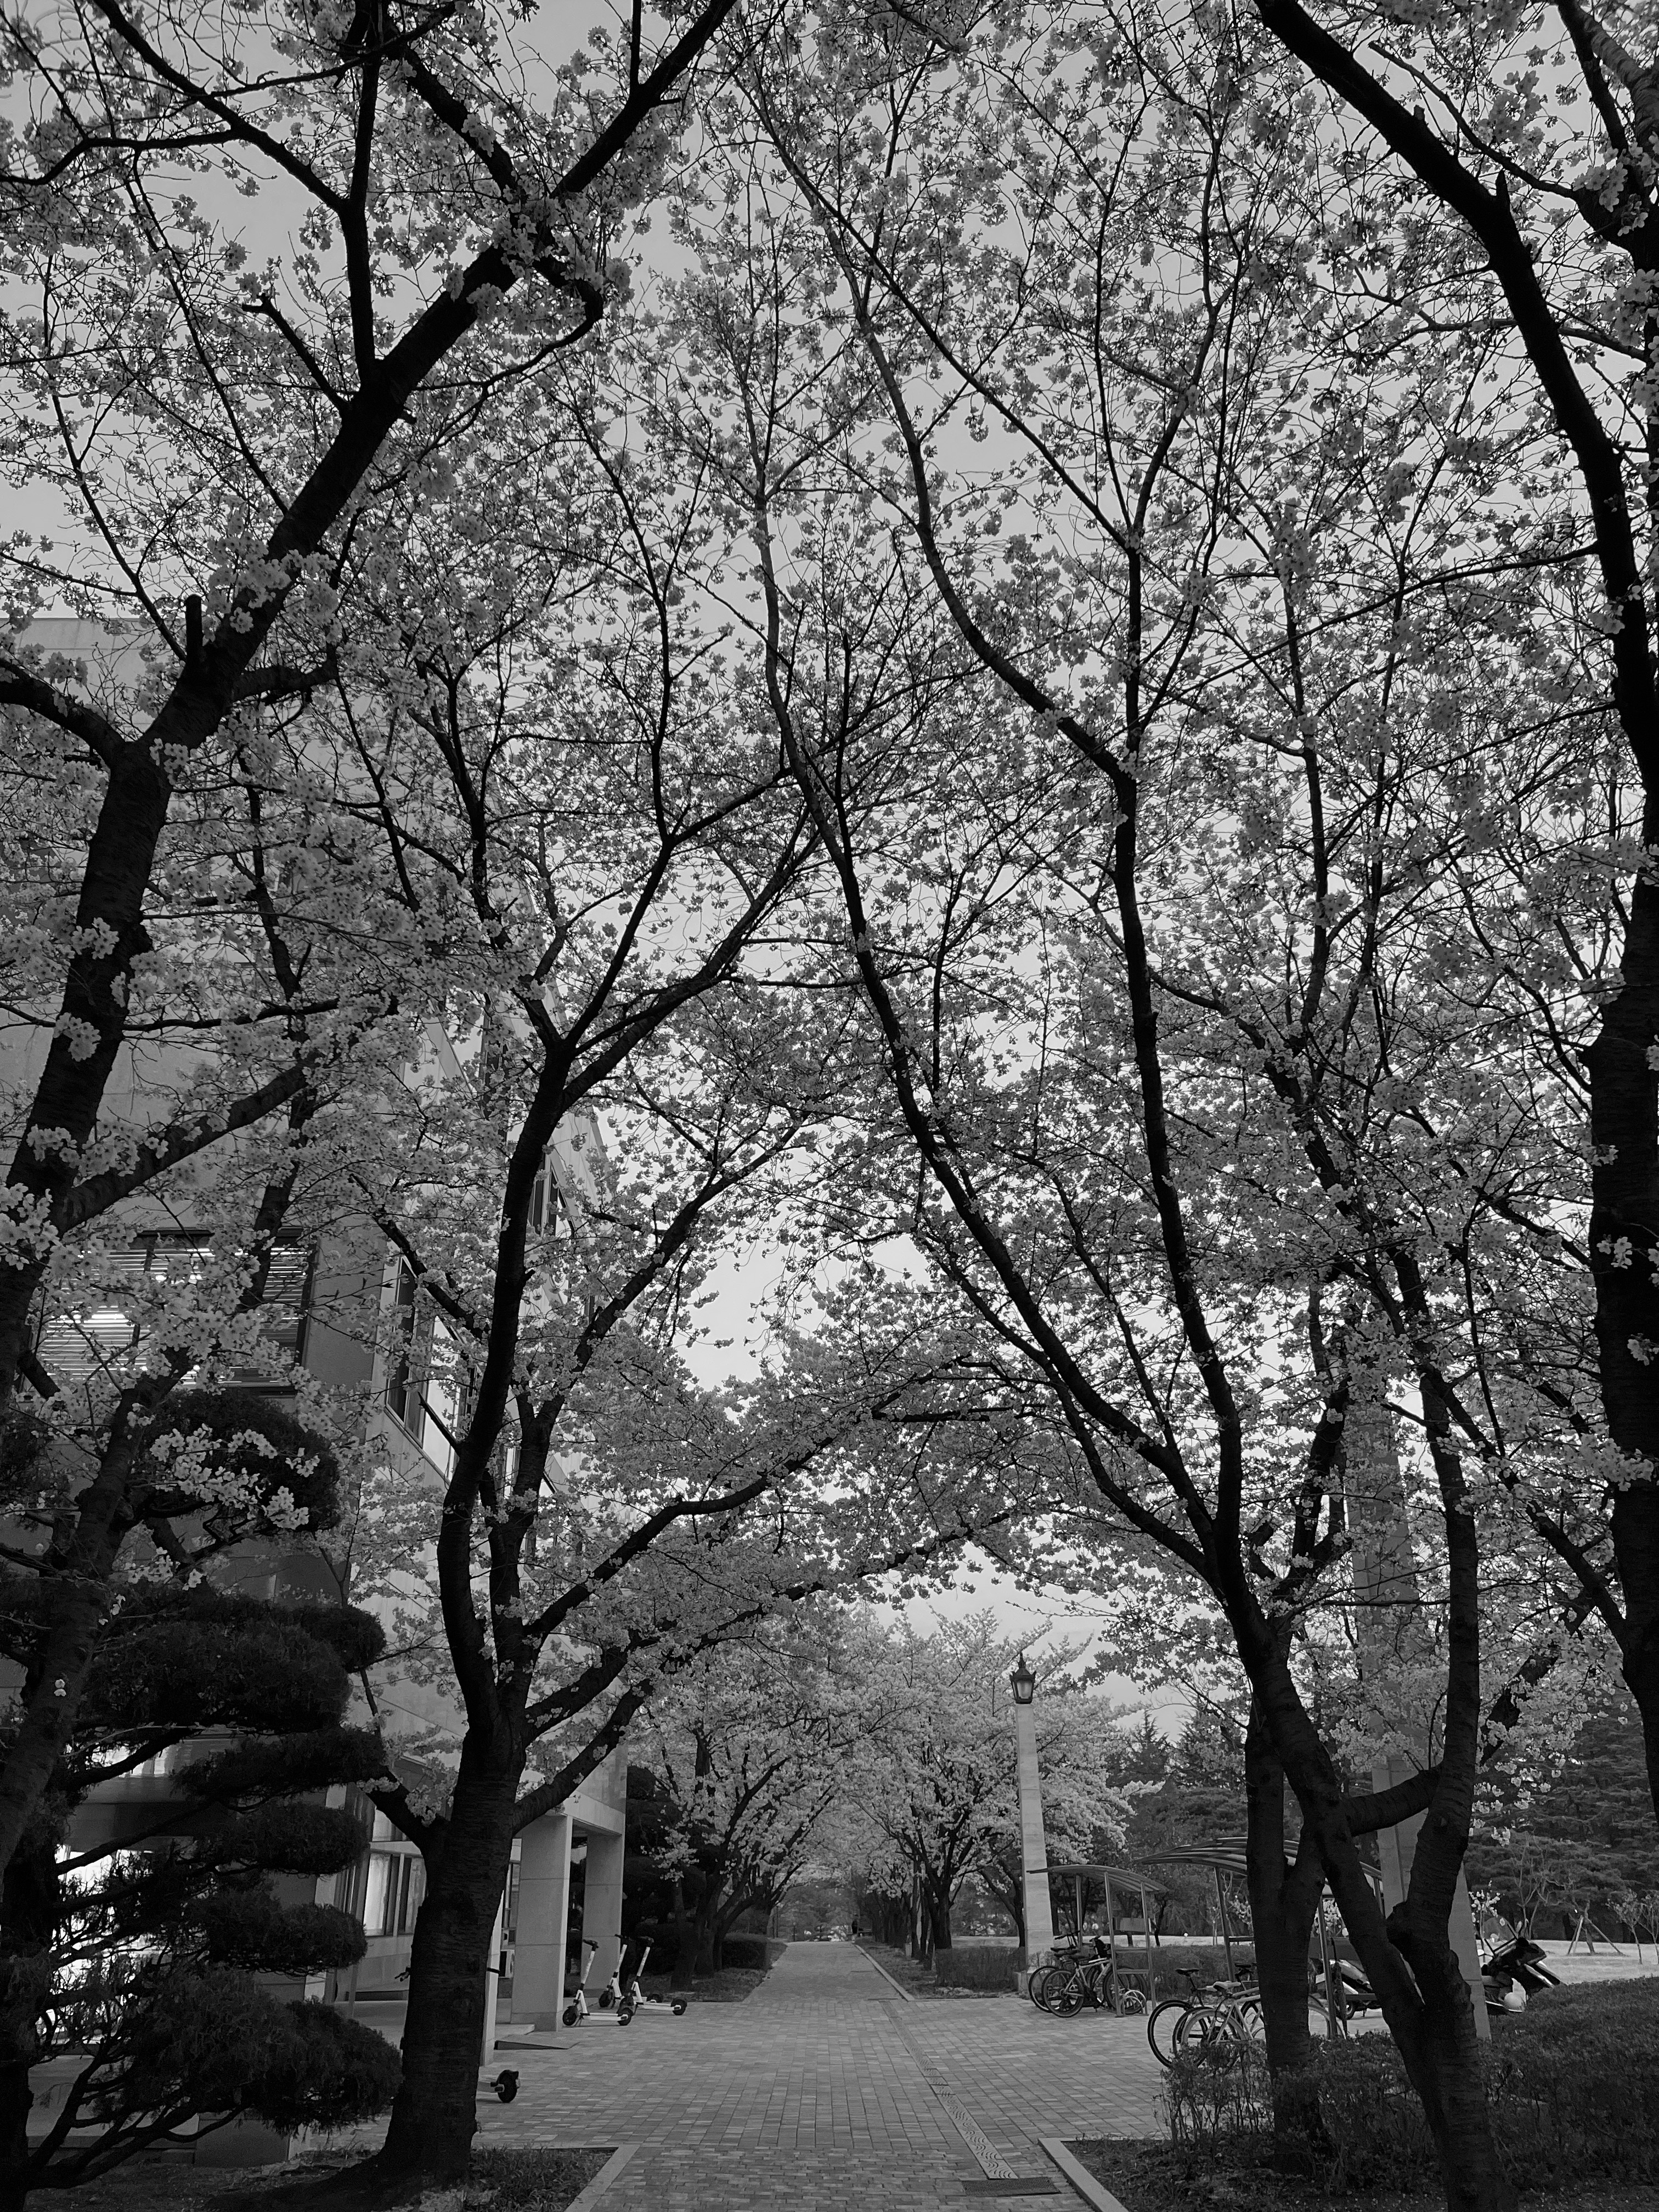
\includegraphics[width=0.2\linewidth]{../images/input/gray6.jpg}}

    \caption{Additional Input Images}
\end{figure}

Problem 1에서 사용한 Color 이미지들과 이를 흑백으로 변환한 이미지들을 추가로 사용한다.
추가로 사용하는 흑백 이미지는 위와 같다.
Problem 1에서 기존 사용하였던 이미지들은 위에서 확인 가능하다.
직접 촬영하여 추가한 사진의 경우 OpenCV를 통하여 GrayScale로 변환 후 저장하여 사용한다.

\subsection*{Output Images}

다음은 실행 결과 이미지와 해당 이미지의 전후 각 채널에 대한 시각화를 진행한 결과이다. (시각화되지 않은 실행 결과 이미지들은 \code{images/output/problem2}에서 확인할 수 있다.)

\begin{figure}[htbp]
    \centering

    \subfloat[color1.jpg]{\includegraphics[width=0.48\linewidth]{../images/output/problem2/visualization/visualization_color1.png}}
    \hspace{1pt}
    \subfloat[color2.jpg]{\includegraphics[width=0.48\linewidth]{../images/output/problem2/visualization/visualization_color2.png}}

    \medskip

    \subfloat[color3.jpg]{\includegraphics[width=0.48\linewidth]{../images/output/problem2/visualization/visualization_color3.png}}
    \hspace{1pt}
    \subfloat[color4.jpg]{\includegraphics[width=0.48\linewidth]{../images/output/problem2/visualization/visualization_color4.png}}

    \medskip

    \subfloat[color5.jpg]{\includegraphics[width=0.48\linewidth]{../images/output/problem2/visualization/visualization_color5.png}}
    \hspace{1pt}
    \subfloat[color6.jpg]{\includegraphics[width=0.48\linewidth]{../images/output/problem2/visualization/visualization_color6.png}}

    \caption{Output Color Images}
\end{figure}

\begin{figure}[htbp]
    \centering

    \subfloat[gray1.jpg]{\includegraphics[width=0.35\linewidth]{../images/output/problem2/visualization/visualization_gray1.png}}
    \hspace{1pt}
    \subfloat[gray2.jpg]{\includegraphics[width=0.35\linewidth]{../images/output/problem2/visualization/visualization_gray2.png}}

    \medskip

    \subfloat[gray3.jpg]{\includegraphics[width=0.35\linewidth]{../images/output/problem2/visualization/visualization_gray3.png}}
    \hspace{1pt}
    \subfloat[gray4.jpg]{\includegraphics[width=0.35\linewidth]{../images/output/problem2/visualization/visualization_gray4.png}}

    \medskip

    \subfloat[gray5.jpg]{\includegraphics[width=0.35\linewidth]{../images/output/problem2/visualization/visualization_gray5.png}}
    \hspace{1pt}
    \subfloat[gray6.jpg]{\includegraphics[width=0.35\linewidth]{../images/output/problem2/visualization/visualization_gray6.png}}

    \caption{Output Gray Images}
\end{figure}

\subsection*{Discussion - Brightness \& Colors}

Histogram Equlization은 Linear한 Cumulative Histogram Function을 만드는 Transformation이다.
밝기는 픽셀값이 높을 수록 밝다고 인식하게 되는데, Linear하도록 Transformation이 진행되다 보니, 원래 밝았던 이미지는 어두워지는 경향을, 어두웠던 이미지는 밝아지는 경향을 보인다.
이는 Cumulative Histogram Function의 오목함과 볼록함을 통해 해석할 수 있을 것으로 생각된다.

색감의 경우, 밝기와 마찬가지로 각 RGB 채널의 픽셀값에 의하여 해당 픽셀이 더 붉어보이거나, 초래보이거나, 푸르러보인다.
앞서 이야기했듯이 Linear하도록 만들다 보니, 결국 덜 붉었던 부분은 더 붉도록, 덜 초래보이던 부분은 더 초래보이도록, 덜 푸르르던 부분은 더 푸르게 보이도록 만들게 된다.

결론적으로, Histogram Equlization은 이미지를 전반적으로 모든 부분에서 균일하게 보일 수 있도록 처리하는 방법이라고 생각할 수 있다.
이와 더불어, 전체 이미지의 대비가 올라가 이미지 내 물체들의 구분성도 높아지는 효과를 가져오게 된다.

\subsection*{Discussion - Improvement}

\code{color5.jpg}나 \code{gray5.jpg}의 시각화 결과를 볼 경우, 어두운 밤에 찍힌 이미지이다보니 낮은 픽셀값의 분포가 높아, Equlization 이후에는 낮은 픽셀값에서 비교적 너무 Discrete한 경향을 보인다.
이미지로 보았을 때, 지나치게 밝기가 올라가면서 전체적인 이미지를 확인하기 힘든데, 이런 Discrete한 구간에 대한 완화된 Equlization을 적용해, Equlization 이후 이를 개선할 수 있을 것으로 생각된다.

\end{document}
